\begin{frame}
    \frametitle{Further Analysis of Sample K}
    % a comment
    \begin{columns}
            \column[t]{5cm}
            \begin{figure}
                    \begin{center}
                            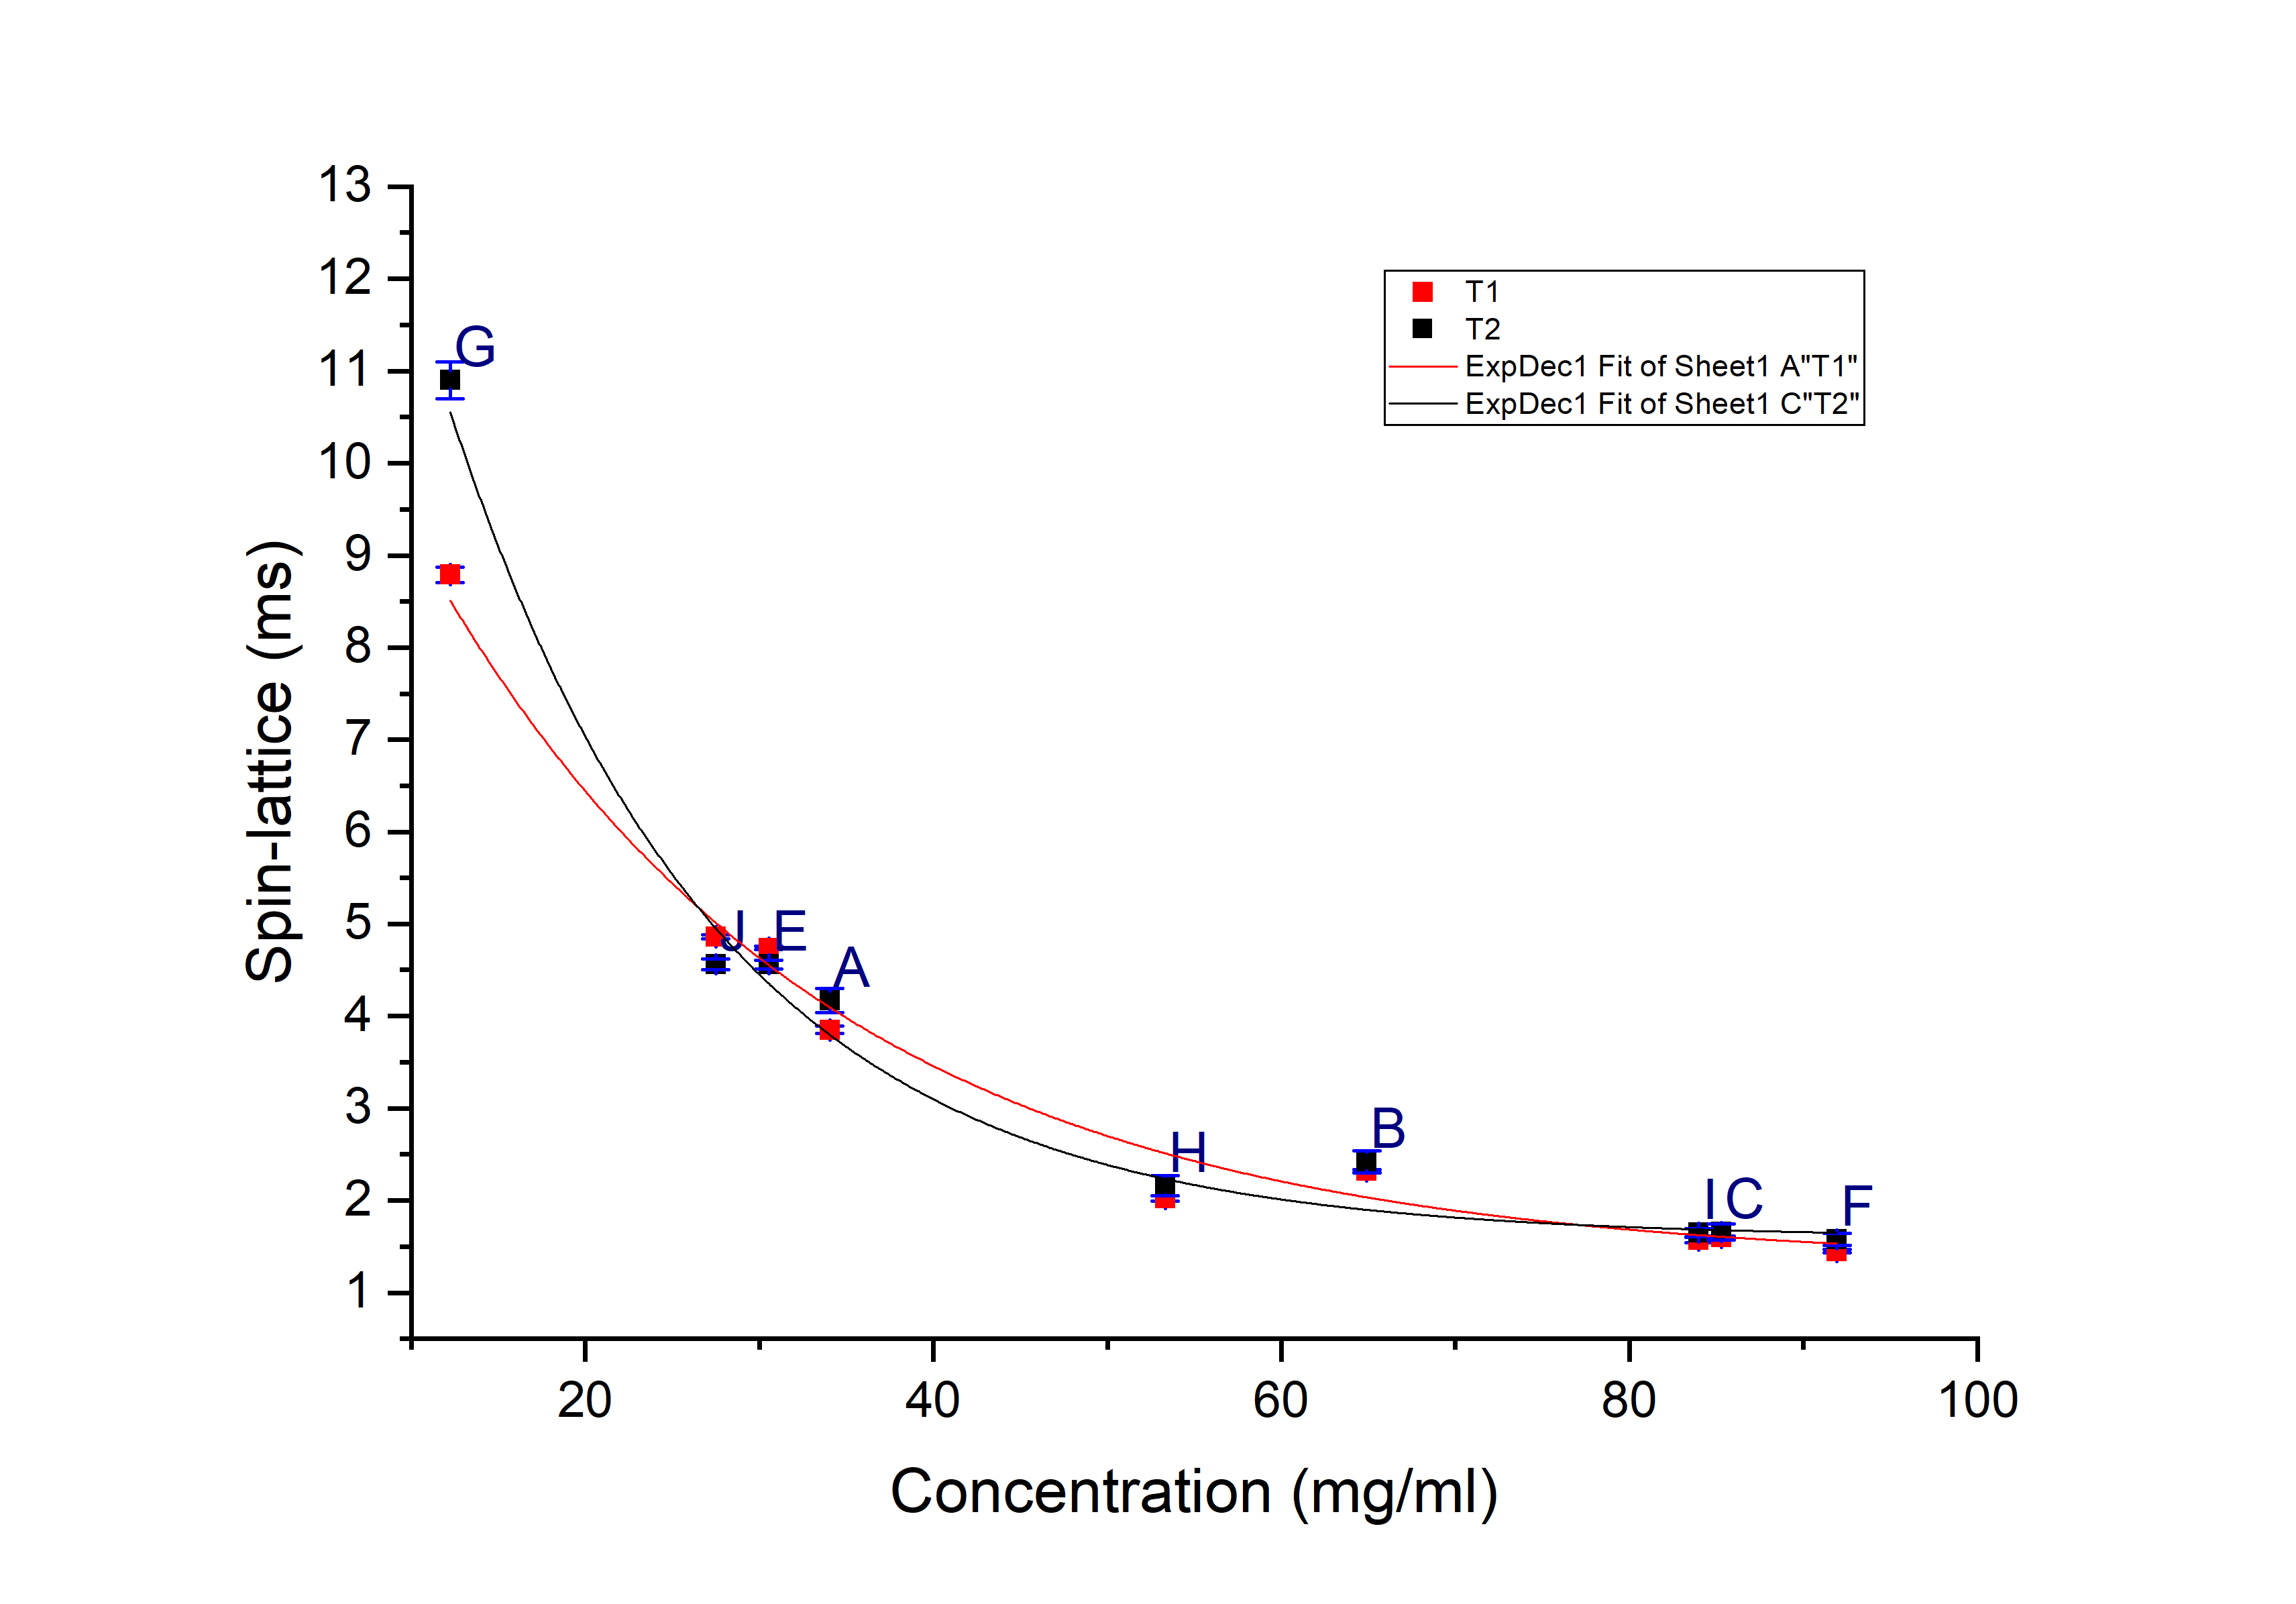
\includegraphics[scale=0.17]{./images/figures/res_k/res_w-out_k.jpg}
                    \end{center}
                            \caption{Fit without Sample K}
                    \label{fig:w-out_k}
            \end{figure}
            \column[t]{5cm}
                \begin{itemize}
                        \item The $T_1$ fit indicates a concentration of 37.9
                        \item The $T_2$ fit indicates a concentration of 33.4
                \end{itemize}
            Superficial literature review revealed no indication that this range of concentrations should behave differently.
          \end{columns}
\end{frame}